\section{Why learn C++?}
\begin{itemize}
    \item Popular: 
        \begin{itemize}
            \item Lots of code is still written in C++.
            \item Programming language popularity indexes ranks C++ high.
            \item Active community, Github, Stack overflow.
        \end{itemize}

    \item Relevant: 
        \begin{itemize}
            \item Windows, Linux, MaxOSX, Photoshop, Illutstrator, MySQL, MonggoDB.
            \item Amazon, Apple, Microsoft, PayPal, Google, Facebook, MySQL, Oracle, HP, IBM, more... 
            \item VR, Unreal Engine, Machine learning, networking \& telecom, more...
        \end{itemize}
    
    \item Powerful: 
        \begin{itemize}
            \item Super-fast, scalable, portable.
            \item Supports both procedural and object-oriented programming.
        \end{itemize}
    
    \item Good career opportunities:
        \begin{itemize}
            \item C++ skills always in demand.
            \item C++ = Salary++.
        \end{itemize}
\end{itemize}



%----------------------------------------------------------------------------------------
\section{Modern C++ and the C++ standard}
\begin{multicols}{2}
    \begin{itemize}
        \item Early 1970s: C programming language; Dennis Ritchie.
        \item 1979: Bjarne Stroustrup; 'C with classes'.
        \item 1983: Name changed to C++.
        \item 1989:First commercial release. 
        \item 1998: C++98 Standard.
        \item 2003: C++03 Standard. 
        \item 2011: C++11 Standard. 
        \item 2014: C++14 Standard. 
        \item 2017: C++17 Standard. 
    \end{itemize}
\end{multicols}

\subsection{Modern C++ and C++ Standard}
\begin{itemize}
    \item Classical C++: Pre C++11 Standard. 
    \item Modern C++: 
        \begin{itemize}
            \item C++11: Lots of new features. 
            \item C++14: Smaller changes. 
            \item C++17: Simplification. 
        \end{itemize}
\end{itemize}


%----------------------------------------------------------------------------------------
\section{How does it all work?}
\begin{itemize}
    \item Use non-ambiguous instructions. 
    \item Programming language: source code, high level, for humans.
    \item Editor: text editor. \emph{.cpp} and \emph{.h} files.
    \item Binary or other low level representation: object code for computers. 
    \item Compiler: Translates from high-level to low-level. 
    \item Linker: links together our code with other libraries, creates \emph{.exe}.
    \item Testing and debugging: finding and fixing program errors.
\end{itemize}

\subsection{The C++ build process}
\begin{figure}[H]
    \centering
    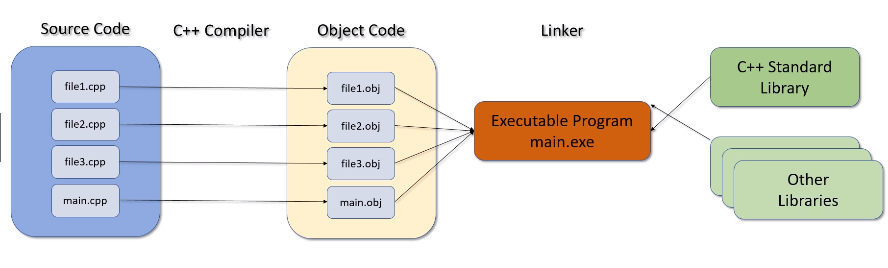
\includegraphics[width=\textwidth]{\figs/cppbuilding}
\end{figure}

\subsection{Integrated Development Environments (IDEs)}
\begin{multicols}{2}
    \begin{itemize}
        \item Editor.
        \item Compiler.
        \item Linker.
        \item Debugger. 
        \item Keep everything in sync. 
    \end{itemize}
\end{multicols}
\subsubsection{IDEs}
\begin{multicols}{3}
    \begin{itemize}
        \item CodeLite. 
        \item Code::Blocks.
        \item NetBeans.
        \item Eclipse.
        \item CLion.
        \item Dev-C++.
        \item KDevelop.
        \item Visual Studio.
        \item Xcode.
    \end{itemize}    
\end{multicols}


%----------------------------------------------------------------------------------------
